\pdfoutput=1
\synctex=1

\documentclass{article} % For LaTeX2e

%STANDARD PREAMBLE
%https://tex.stackexchange.com/questions/68821/is-it-possible-to-create-a-latex-preamble-header
\usepackage{/Users/mwojno01/Research/Learning/latex_preamble/preamble}


%%% CONTROL SIZE OF BLOCK MATRICES
% Reference: https://tex.stackexchange.com/questions/14071/how-can-i-increase-the-line-spacing-in-a-matrix

\makeatletter
\renewcommand*\env@matrix[1][\arraystretch]{%
  \edef\arraystretch{#1}%
  \hskip -\arraycolsep
  \let\@ifnextchar\new@ifnextchar
  \array{*\c@MaxMatrixCols c}}
\makeatother
 
 % INDICATOR FUNCTIONS
 % Allows us to switch between delta(x,y)
 % or Iverson bracket $[x=y]$ or $[x==y]$
 % or 1_{whatever} ..
 
 %\newcommand{\indicate}[2]{\delta({#1},{#2})}
% \newcommand{\indicate}[2]{[{#1} = {#2}]}
  
 %%% MARKOV RANDOM FIELDS 
\newcommand{\selfpotential}{\phi}
\newcommand{\edgepotential}{\psi}

%%%% HIDDEN MARKOV MODEL
\newcommand{\state}{x}

\begin{document}



\title{Exponential Family} 

\maketitle

\tableofcontents
\newpage

\section{The Exponential Family} \label{sec:ef}

We are interested in the exponential family primarily because it makes inference easier.   When a problem can be cast within the exponential family framework,  inference can be tied to general principles,  and parameter updates often have nice interpretations.    This is true regardless of whether we're doing frequentist inference (such as maximum likelihood) or Bayesian inference.    Bayesian inference with exponential family likelihoods tends to be especially nice,  as all exponential family likelihoods have conjugate priors,  and these are often also in the exponential family \cite{bernardo2009bayesian}. \redfootnote{TODO:  Get clearer on the relationship.  There is a brief discussion on this in \cite{bernardo2009bayesian}.  I am not clear on whether all likelihoods with conjugate priors need to be in the exponential family.}   More complicated models may not be in the exponential family,  but may have exponential family complete conditional distributions;  in such situation,  we can appeal to exponential family formalisms to more easily work out inference schemes for expectation maximization,  variational inference,  or Gibbs sampling.   

\subsection{Definition}
We define an \textit{exponential family} of probability distributions as those distributions whose density has the following form
\begin{align}
\label{eqn:exponential_family}
 p(x \cond \theta) = h(x) \exp \{ \eta(\theta)^T t(x) - a(\theta)\} 
 \end{align}
where we refer to $h$ as the base measure, $\eta$ as the natural parameter, $t$ as the sufficient statistics, and $a$ as the log normalizer.  \redfootnote{TODO: It would be helpful to get more solid on integrating against probability measure here, so that I can set this up in a more precise way, as Jordan does.    He remarks on this somewhere in his exponential family lecture notes.   What also may be helpful is this beautiful excerpt from pp.38 of \cite{wainwright2008graphical}: `` $[...]$ we represent the probability distribution as a density $p$ absolutely continuous with respect to some measure $\eta$.   This base measure $\eta$ might be the counting measure on $\set{0, 1, ..., r-1}$,  in which case $p$ is a probability mass function; alternatively, for a continuous random vector, the base measure $\eta$ could be the ordinary Lebesgue measure on $\R$."}

\begin{remark}{\remarktitle{Non-uniqueness of natural parameter}}
\label{rk:nonuniqueness_of_natural_parameter}
Note from \eqref{eqn:exponential_family} that natural parameters are not unique since,  for example,  $\eta$ could be multiplied by a non-zero constant $c$ if $t(x)$ is divided by $c$. \redfootnote{Are they unique up to scalar multiplication?} Thus,  we should speak of \textit{a} natural parameter,  rather than \textit{the} natural parameter.
\end{remark}

\subsection{Examples}
\subsubsection{Dirichlet distribution}

\begin{example}{(Dirichlet Distribution)} 
\label{ex:dirichlet_as_ef} We can write the density of the Dirichlet distribution in exponential family form:
\begin{align*}
p (\pi \cond\alpha) &= \df{\Gamma(\sum_k \alpha_k)}{\prod_k \Gamma (\alpha_k) } \pi_1^{\alpha_1 -1} \cdot \cdot \cdot \pi_K^{\alpha_K -1} \\
&= \exp \bigg\{ \sum_{k=1}^K (\alpha_k -1) \log \pi_k - \bigg[ \sum_k \log \Gamma (\alpha_k)-  \log \Gamma (\sum \alpha_k) \bigg]  \bigg\}
\end{align*}
with natural parameter $\eta(\alpha) = [\alpha_1 -1, ..., \alpha_K -1]^T$, sufficient statistics $t(\pi) = \log \pi = [\log \pi_1, ..., \log \pi_K]^T$, base measure $h(\pi)=1$, and log normalizer $a(\alpha) =  \sum_k \log \Gamma (\alpha_k ) - \log \Gamma (\sum_k \alpha_k)$. 
\qed 
\end{example} 

For an example of how the natural parametrization can help provide insight into message passing,  see Section \ref{sec:mvn_in_message_passing}.

\begin{remark} The exponential family representation of the Dirichlet, as given in Example \ref{ex:dirichlet_as_ef}, is useful when we want to compute the expectation of a log probability from a Dirichlet distributed probability vector (as happens in the derivation of LDA with variational inference; see my notes on variational inference).  

In those notes,  we see
\begin{align} 
\E [ \log \pi_k] &= \E [t_k(p)] \stackrel{1}{=} \df{\partial}{\partial \eta_k} a(\eta) \nonumber \\
&=\Psi(\alpha_k) -  \Psi(\sum_k  \alpha_k) \label{eqn:expectation_of_log_probability} 
\end{align}
where (1) uses a well-known exponential family property and where $\Psi(\cdot)$ is the first derivative of the $\log \Gamma$ function.   It is known as the \textit{digamma function}.  $\qed$

% See e.g., https://zhiyzuo.github.io/Exponential-Family-Distributions/
\end{remark}

\red{TODO:  Add multivariate Gaussian example,  showing that the natural parameters are the precision $\Sigma^{-1}$ and precision-weighted mean $\Sigma^{-1} \mu$,  as we use this in Section \ref{sec:normal_data_with_non_conjugate_prior} combined with the exponential family formalism to derive the updates to the mean for a Bayesian normal model with conditionally conjugate prior.}




\subsubsection{Truncated normal distribution}

\begin{example}{(Truncated normal distribution)} 
\label{ex:truncated_normal_as_ef} The univariate truncated normal distribution $\TruncatedNormal(\mu,  \sigma^2,  \Omega)$ results when a normal distribution $\N(\mu,  \sigma^2)$ is truncated to some set $\Omega \in \R$. \footnote{For more information on the truncated normal,  see e.g.  \cite{burkardt2014truncated} or \url{http://parker.ad.siu.edu/Olive/ch4.pdf}.}   Note that the parameters $\mu, \sigma^2$ denote the mean and variance of the \textit{parent} normal distribution;  i.e.  if $X \sim \TruncatedNormal(\mu,  \sigma^2,  \Omega)$ then $\E[X] \neq \mu$ (unless $\Omega = \R$). 

If we assume that the truncation set is an interval $\Omega = (a,b)$ for $a,b \in \R$,  then the distribution $\TruncatedNormal(\mu,  \sigma^2,  (a,b))$ has p.d.f.

\begin{align*}
f(x ; \mu,  \sigma^2,  a,  b) = \df{\phi_{\mu, \sigma^2} (x) }{\Phi_{\mu, \sigma^2} (b)  - \Phi_{\mu, \sigma^2} (a) } \indicate{a \leq x \leq b} \labelit \label{eqn:pdf_of_normal_truncated_to_an_interval}
\end{align*} 

where $\phi_{\mu,  \sigma^2}$ and $\Phi_{\mu,  \sigma^2}$ denote the pdf and cdf,  respectively,  of a univariate normal distribution with mean $\mu$ and variance $\sigma^2$.   

If we write
\begin{align*}
f(x ; \mu,  \sigma^2,  a,  b) & = K \df{1}{\sqrt{2 \pi \sigma^2}} \exp \bp{-\half \df{(x-\mu)^2}{\sigma^2}}  \indicate{a \leq x \leq b} \\
& = K \df{1}{\sqrt{2 \pi \sigma^2}} \exp \bp{ - \frac{1}{2 \sigma^2} x^2 + \frac{\mu}{\sigma^2} x  + \frac{\mu^2}{\sigma^2}  - \log \sigma}  \indicate{a \leq x \leq b} 
\end{align*} 
where $K := \big( \Phi_{\mu, \sigma^2} (b)  - \Phi_{\mu, \sigma^2} (a) \big)^{-1}$,  then we see that see that  $\TruncatedNormal(\mu,  \sigma^2,  (a,b))$ belongs to the exponential family \eqref{eqn:exponential_family} where,  in this case,  we have natural parameter $\eta = (- \frac{1}{2 \sigma^2},  \frac{\mu}{\sigma^2})^T$,  sufficient statistics function $t(x) = (x^2,  x)^T$,  base measure $h(x) =  \frac{1}{\sqrt{2 \pi}}  \indicate{a \leq x \leq b}$,  and log normalizer $a(\theta) = \log K + \frac{\mu^2}{\sigma^2} - \log \sigma$.
\qed
\end{example}

\begin{remark}
The truncated normal distribution differs from the normal distribution only in its base measure $h(x)$ and log normalizer $a(\theta)$.  The natural parameter $\eta$ and sufficient statistics function $T(x)$ are identical.   Thus,  knowing $\eta$ and $T(x)$ is not sufficient to determine the form of the probability distribution.
\end{remark}


\subsubsection{Inverse Gamma distribution}

\begin{example}{(Inverse Gamma Distribution)} 
\label{ex:inverse_gamma_as_ef} The Inverse Gamma distribution is the distribution of the reciprocal of a Gamma random variable.\footnote{The density of the inverse gamma can easily be obtained from the gamma density by defining the transformation $Y = \df{1}{X} := g(X)$ and then applying the change of variables formula,  $f_Y(y) = f_X (g^{-1}(y)) | \df{d}{dy} g^{-1}(y)|$.}  We can write the density of the Inverse Gamma $\InverseGamma(\alpha,  \beta)$ distribution in exponential family form:
\begin{align*}
p (x \cond \alpha,  \beta) &= \df{\beta^\alpha}{ \Gamma (\alpha) } x^{-\alpha -1} \exp \bigg(- \df{\beta}{x} \bigg) \\
&= \exp \bigg\{ (-\alpha - 1) \log x + (- \beta) \frac{1}{x} + \log \df{\beta^\alpha}{\Gamma(\alpha)} \bigg\}
\end{align*}
with natural parameter $\eta(\alpha) = [-\alpha-1,  -\beta]^T$, sufficient statistics $t(x) = [\log x ,  \frac{1}{x}]^T$, base measure $h(x)=1$, and log normalizer $a(\alpha,  \beta) =  \log \frac{\beta^\alpha}{\Gamma(\alpha)} $. 
\qed 
\end{example} 

\subsubsection{Inverse Wishart distribution}

\begin{example}{(Inverse Wishart distribution)} 
\label{ex:inverse_wishart_as_ef} The Inverse Wishart distribution (Section \ref{sec:inverse_wishart_distribution}) is the distribution of the inverse of a Wishart random variable.   We can write the density of the Inverse Wishart $\InverseWishart(\+\Psi,  \nu)$ distribution in exponential family form:
\begin{align*}
p (\+X  \cond \+\Psi,  \nu) & \stackrel{1}{=} C(\+\Psi,  \nu) \; | \+X | ^{-(\nu + p + 1)/2} \exp \bigg\{ -\half \tr (\+\Psi \+X^{-1} ) \bigg\} \\
& = \exp \bigg\{ \frac{-(\nu + p + 1)}{2}  \log | \+ X | \;  -\half \tr (\+\Psi \+X^{-1} )  \; + \log  C(\+\Psi,  \nu)   \bigg\} \\
& \stackrel{2}{=} \exp \bigg\{ \frac{-(\nu + p + 1)}{2}  \log | \+ X | \;  -\half  \ds\sum_{i,j=1}^p \+\Psi_{ij} \+X^{-1}_{ij} \; + \log  C(\+\Psi,  \nu)   \bigg\} 
\end{align*}
Equation (1) gives the standard representation of the $\InverseWishart(\+\Psi,  \nu)$ density,  where   $C(\+\Psi,  \nu)$ is the normalizing constant,  $| \cdot |$ refers to the determinant,  $\+X,  \+\Psi \in \R^{p \times p}$ are positive definite matrices,  and $\nu > p-1$.    Equation (2) uses the fact that the trace of a matrix product behaves like a dot product \eqref{eqn:trace_of_matrix_product}.      


As we see from the last line,  in the exponential family representation,  we have natural parameter $\eta = [\frac{-(\nu + p + 1)}{2},  \; -\half \vectorize (\+\Psi)]^T$, sufficient statistics $t(\+X) = [\log | \+X | , \vectorize (\+X^{-1})]^T$, base measure $h(\+X)=1$, and log normalizer $ \log  C(\+\Psi,  \nu)$.   
\qed 
\end{example} 

%{eqn:trace_of_matrix_product}

\subsubsection{Hidden Markov Models} 

\begin{example}{(Hidden Markov Models)} 
A  hidden Markov model (HMM) is a tool for representing probability distributions over sequences of observations.  The HMM assumes that the observation at time $t$ was generated by some process whose state $\state_t$ is hidden from the observer.  Moreover, it assumes that the sequence of states satisfies the \textit{Markov property}:  conditional on the current state $\state_t$, its future and past hidden states are independent.  Finally, there is a Markov property on outputs:  conditional on the current state $\state_t$, the output $y_t$ is independent of all other hidden states and outputs.\redfootnote{I might have lifted this paragraph overviewing HMM's from somewhere; check into that.}

% Note: No need to introduce the Bayesian hidden markov model here; we're just showing that the complete data likelihood is in the
% exponential family.
%
%The full generative model over the parameters, hidden state sequence $\state_{1:T}$ and observation sequence $y_{1:T}$ is
%
%\begin{align*}
%\pi &\sim \text{Dir}(\alpha^\pi) & A_k &\iid \text{Dir}(\alpha^{A_k})  & \phi_k &\iid p(\phi_k \cond \beta) \\
%\state_1 &\sim \pi & \state_{t+1} &\sim A_{\state_t} & y_t &\sim p(y_t \cond \phi_{z_t})
%\end{align*}
 
The the \textit{complete data likelihood} for the HMM is given by

\begin{align}
 p(\state_{1:T}, y_{1:T} \cond \theta) &=  p(\state_1 \cond \theta)  p(y_1 \cond \state_1, \theta) \ds\prod_{t=2}^T p(\state_t \cond \state_{t-1}, \theta) p(y_t \cond \state_t, \theta) \nonumber \\
 &=  p(\state_1 \cond \pi) p(y_1 \cond \state_1, \phi) \ds\prod_{t=2}^T p(\state_t \cond \state_{t-1}, A) p(y_t \cond \state_t, \phi)   \nonumber \\
 &= \pi_{\state_1}  \; \ds\prod_{t=2}^T A_{\state_{t-1}, \state_t} \ds\prod_{t=1}^T p(y_1 \cond \phi_{\state_t}) \label{eqn:hmm_cdl_compact}
 \end{align}
 
where we have defined 

\begin{itemize}
\item $y_{1:T}=(y_1, ..., y_T)$ observed sequence
\item $\state_{1:T} =(\state_1, ...., \state_T)$: hidden state sequence ($\state_t \in \{1,...,K \}$) 
\item $\pi = \{ \pi_k \}, \pi_k = P(\state_1 = k)$: initial state distribution
\item $A=\{A_{kk'}\}, A_{kk'} = P(\state_t= k' \cond \state_{t-1}=k):$ state transition probability matrix 
\item $\phi = (\phi_k)_{k=1}^K$ a set of parameters, each governing an output distribution (also called emissions distribution) associated to each hidden state; that is, $ P(y_t \cond \state_t=k) = P(y_t \cond \phi_k)$. 
\item $\theta = (\pi, A, \phi)$: model parameters
\end{itemize}


We can write the complete data likelihood \eqref{eqn:hmm_cdl_compact} as
\begin{align}
p(\state_{1:T}, y_{1:T} \cond \theta) &=  \exp\bigg \{ \log p(\state_1 \cond \pi) + \ds\sum_{t=2}^T \log p(\state_t \cond \state_{t-1}, A) +  \ds\sum_{t=1}^T \log p(y_t \cond \state_t, \phi) \bigg\}  \nonumber \\
&= \exp \bigg \{ \log \pi_{\state_1}  + \ds\sum_{t=2}^T \log A_{\state_{t-1}, \state_t} + \ds\sum_{t=1}^T \log p(y_1 \cond \phi_{\state_t}) \bigg\} \nonumber \\
&=  \exp\bigg \{  \ds\sum_{k=1}^K \state_1^k \log \pi_k + \ds\sum_{t=2}^T \ds\sum_{k, k'=1}^K \state_{t-1}^k \state_t^{k'} \log A_{kk'} + \ds\sum_{t=1}^T \ds\sum_{k=1}^K \state_t^k \log p(y_t \cond \phi_k)  \bigg\} \label{eqn:hmm_ef_form}
\end{align}

where we have defined
\[ \state_t^k =  
\begin{cases}	  
1, & \text{if the latent state at time $t$ is $k$} \\
0, & \text{otherwise}
\end{cases} \]

and \eqref{eqn:hmm_ef_form} shows that the HMM is in the exponential family, so long as the emissions distributions are. 
The sufficient statistics for $\log \pi_k$ are $\state_1^k$, and the sufficient statistics for $\log A_{kk'}$ are $\sum_{t=2}^T \state_{t-1}^k \state_t^{k'}$. 

\end{example}

\subsection{i.i.d samples from an exponential family}
If $\+x=(x_1, ..., x_n)$ are n independent samples from the same exponential family, then 
\begin{align}
\label{eqn:exponential_family_iid}
 p(\+x \cond \theta) = \ds\prod_{i=1}^n h(x_i) \exp \big\{ \eta(\theta)^T \sum_{i=1}^n t(x_i) - n \,a(\eta(\theta))\big\} 
 \end{align}

\section{Exponential Family: Maximum Likelihood Estimation} \label{sec:ml_with_ef}

The goal for maximum likelihood is to determine the parameter
\begin{equation}
\label{eqn:ml}
\theta_{ML} = \argmax_\theta  \, \log p(\+x \cond \theta) 
\end{equation}

Let us assume that $\+x=(x_1, ..., x_n)$ are i.i.d observations  from a fixed exponential family, so that the likelihood has form \eqref{eqn:exponential_family_iid}.  Let us compute the gradient with respect to the natural parameter $\eta$ of $\ell(\eta) := \log p(\+x \cond \eta)$

\[ \nabla_\eta \ell(\eta) = \ds\sum_{i=1}^n t(x_i) - n \; \nabla_\eta a(\eta) \]

Setting the gradient to zero, we obtain

\[ \nabla_\eta a(\eta) = \df{1}{n}  \ds\sum_{i=1}^n t(x_i) \]

But $\nabla_\eta a(\eta) = \E [t(X)]$ \cite{jordan_ef}.  Thus, we should set $\theta_{ML}$ such that

\[ \mu(\theta_{ML}) = \df{1}{n} \ds\sum_{i=1}^n t(x_i) \]
where $\mu := \E[t(x)]$ refers to the mean parametrization of the likelihood. \redfootnote{TODO: This switching of parameterization should be handled much more explicitly.}

 \section{Exponential Family: Expectation Maximization} \label{sec:em_with_ef}

Some models have latent variables associated with each observation, and so maximum likelihood is not possible.  Let us see how expectation maximization looks when the complete data likelihood is in the exponential family.

The expectation maximization algorithm is 
\begin{equation}
\label{eqn:em_algorithm_appendix}
 \+\theta^{(t+1)} =  \text{argmax}_{\+\theta} \; \E_{p(\+z \cond \+x , \+\theta^{(t)})} \bigg[ \ln p(\+x, \+z \cond \+\theta) \bigg] 
 \end{equation}

We see how this plays out in the exponential family by following the logic of Section \ref{sec:ml_with_ef}.   Let us assume that $(\+x, \+z)=((x_1,z_1), ..., (x_n, z_n))$ are n independent samples from the same exponential family, where $\+x$ is observed data and $\+z$ is unobserved data.
Moreover, let us assume that the complete data likelihood is in the exponential family

\begin{align}
\label{eqn:exponential_family_complete_data_likelihood}
 p(\+x, \+z \cond \theta) = \ds\prod_{i=1}^n h(x_i, z_i) \exp \big\{ \eta(\theta)^T \sum_{i=1}^n t(x_i, z_i) - n \,a(\eta(\theta))\big\} 
 \end{align}

Here we want to find $\+\theta$ to optimize 
\[ f(\+\theta) =  \E_{p(\+z \cond \+x , \+\theta^{(t)})} \bigg[ \ln p(\+x, \+z \cond \+\theta) \bigg] \]

Following the logic of Section \ref{sec:ml_with_ef}, we determine that we should select $\theta^{(t+1)}$ such that
\[ \mu(\theta^{(t+1)}) = \df{1}{n} \ds\sum_{i=1}^n   \E_{p(\+z \cond \+x , \+\theta^{(t)})} t(x_i, z_i) \]
where $\mu := \E[t(x_1,z_1)]$ refers to the mean parametrization of the likelihood.

This is why an EM iteration is often described and/or implemented as performing maximum likelihood with the expected sufficient statistics.

\red{TODO: But is EM \textit{always} equivalent to performing ML with ESS's? Or is this ONLY true if I'm working within the exponential family?  I need to read up some more on EM theory.}

\red{TODO: Check this section, especially with respect to the fact that I am dealing with three parametrizations here - $\mu, \theta, \nu$; that is, mean, arbitrary, and natural, respectively.  Really the core problem is that it's not sufficiently clear in how head how and when reparametrizations affect things.}
 
 \section{Conjugate and semi-conjugate models} \label{sec:conjugate_exponential_family_models}
 
Conjugacy can be defined as follows \cite{gelman2013bayesian}. If $\mathcal{F}$ is a class of sampling distributions and $\mathcal{P}$ is a class of prior distributions for $\theta$, then the class $\mathcal{P}$ is \textit{conjugate} for $\mathcal{F}$ if
\[  p(\theta \cond y ) \in \mathcal{P} \; \text{for all} \; p(\cdot \cond \theta) \in \mathcal{F} \; \text{and} \; p(\cdot) \in \mathcal{P} \]

Conditional conjugacy (sometimes called semi-conjugacy) can be defined similarly  \cite{gelman2013bayesian}.  If $\mathcal{F}$ is a class of sampling distributions and $\mathcal{P}$ is a class of prior distributions for $\theta \cond \phi$, then the class $\mathcal{P}$ is \textit{conditionally conjugate} for $\mathcal{F}$ if
\[  p(\theta \cond \phi, y) \in \mathcal{P} \; \text{for all} \; p(\cdot \cond \theta, \phi) \in \mathcal{F} \; \text{and} \; p(\cdot \cond \phi) \in \mathcal{P} \]

\begin{remark}{\remarktitle{On Conditional conjugacy}}
In other words,  a family of prior distributions for a parameter is called conditionally conjugate if the conditional posterior distribution (often called the \textit{complete conditional}),  given the data and all other parameters in the model,  is also in that class  \cite{gelman2006prior}. \redfootnote{Add some notes,  or refer back to notes from regular conjugacy (once they're created),  pointing out how this definition can be vapid,  and also how conjugate priors are not unique. }    In Section \ref{sec:normal_data_with_non_conjugate_prior}, we give perhaps the simplest example of a conditionally conjugate model.
\qed
\end{remark}
 
 Why are conjugate and conditionally conjugate models of interest?  The posterior distributions for conditionally conjugate models are easily approximated with Gibbs sampling or Mean Field Variational Inference -- the former samples from the complete conditional,  whereas the latter takes variational expectations with respect to the natural parameter of the complete conditional.   
 
 \subsection{Univariate normal model}
 
\subsubsection{Example:  Normal prior on mean of univariate Gaussian with known covariance}

\red{TODO: Fill in}

\subsubsection{Example:  Inverse gamma prior on the variance of a univariate Gaussian with known mean}

\begin{proposition} \label{prop:bayes_univariate_normal_with_known_mean}
Consider the Bayesian univariate normal model with known mean $\mu$ and random variance $\sigma^2$
\begin{align*}
\sigma^2 &\sim \IG (\alpha_0,  \beta_0) \\
y_i \cond \mu,  \sigma^2 &\iid \N (\mu,  \sigma^2),  \quad i=1,...,n \\
\labelit \label{eqn:bayesian_uvn_known_mean}
\end{align*}
where $\IG$ denotes the Inverse Gamma distribution.


The posterior distribution for  \eqref{eqn:bayesian_uvn_known_mean} is given by 
\begin{align*}
\sigma^2 \cond \+y,  \mu & \sim \N(\alpha_n,  \beta_n )
\intertext{where}
\alpha_n & =  \alpha_0 + \half\, n\\
\beta_n & = \beta_0 + \half  \ds\sum_{i=1}^n (x_i - \mu)^2 
\labelit \label{eqn:posterior_variance_uvn_fixed_mean}
\end{align*}

\end{proposition}

\begin{proof}

We have 
\begin{align*}
p(\sigma^2 \cond \+y,  \mu) &\stackrel{1}{\propto}  \explaintermbrace{prior}{ p(\sigma^2)} \quad \explaintermbrace{likelihood}{ \ds\prod_{i=1}^n p(y_i \cond \mu,  \sigma^2)} \\
& \stackrel{2}{\propto} \explaintermbrace{prior}{(\sigma^2)^{-\alpha_0 - 1} \exp \big\{ -\df{\beta_0}{\sigma^2} \big\}} \quad  \explaintermbrace{likelihood}{(\sigma^2)^{-n/2}  \,  \exp \big\{ -\df{1}{2\sigma^2}  \ds\sum_{i=1}^n (y_i - \mu)^2 \big\}}  \\
& \stackrel{3}{\propto} (\sigma^2)^{- (\alpha_0 + n/2) - 1} \exp \bigg\{ -\df{\beta_0 + \half \sum_{i=1}^n (x_i - \mu)^2}{\sigma^2} \bigg\}
\end{align*}
where (1) is by Bayes rule (and conditional independence of the observation model),  (2) fills in the pdfs,  and (3) combines like terms so as to look like an Inverse Gamma density.
\end{proof}

\begin{remark}{\remarktitle{Reparametrizing the inverse gamma prior for greater interpretability}}  
\label{rk:inverse_gamma_prior_with_hoff_parametrization}
Peter Hoff \cite{hoff2009first} (pp.74) suggests parametrizing the prior as 
\[ \sigma^2 \sim \IG (\nu_0,  \, \nu_0 \,  \sigma^2_0 / 2) \\ \]
for greater intepretability.   In this case,  we find that the posterior $IG$ parameters are given by
\begin{align*}
\alpha_n & =  \half ( \nu_0 + n )\\
\beta_n & =  \half ( \nu_0 \, \sigma_0^2 + n \, \text{MSE}  )
\intertext{where the mean squared error $\text{MSE}$ is defined by}
\text{MSE} & :=  \df{1}{n} \ds\sum_{i=1}^n (y_i - \mu)^2 
\end{align*}
So $\eta_0$ plays the role of a prior sample size and $\sigma^2_0$ plays the role of the variance within that prior sample. 
% \eqref{eqn:bayesian_uvn_known_mean}
\qed
\end{remark}

 
 
\subsection{Multivariate normal model}
 
\subsubsection{Example:  Normal prior on mean of multivariate Gaussian with known covariance}  \label{sec:normal_prior_on_mvn_with_known_covariance}
 
 
\red{TODO.   Note that in Section \ref{sec:Bayesian_linear_regression_with_normal_prior},   I've already written up a self-enclosed argument for Bayesian linear regression;  some of that argument can likely be factored out to here.}

\subsubsection{Example:  Inverse Wishart prior on covariance matrix of multivariate Gaussian with known mean} \label{sec:inverse_wishart_prior_on_mvn_with_known_mean}
 
Here we will show that the Inverse Wishart is a conjugate prior for the covariance of a multivariate normally distributed random variable with known mean.

This situation comes up 

\begin{example}{\remarktitle{Inverse Wishart prior on the covariance of a  Multivariate Normal sampling model with known mean}} \label{ex:inverse_wishart_prior}



Consider the sampling model for $\+y :=(\+y_1, ....,\+y_n) \iid \N_d(\+\mu,  \+\Sigma)$
\begin{align}
p\+(y \cond \+\mu, \+\Sigma) & \propto | \+\Sigma |^{-n/2} \exp \bb{ -\df{1}{2} \ds\sum_{i=1}^n (\+y_i - \+\mu)^T  \Sigma^{-1} (\+y_i- \+\mu) } \nonumber \\
& = | \+\Sigma |^{-n/2} \exp \bb{ -\df{1}{2} \tr(\+\Sigma^{-1} \+S_\mu)  }\label{eqn:mvn_in_nice_form_for_inverse_wishart_prior}
\end{align}
where $\+S_\mu := \sum_{i=1}^n (\+y_i - \+\mu) (\+y_i - \+\mu)^T$ is the sum of pairwise deviation products,  and where the equality in \eqref{eqn:mvn_in_nice_form_for_inverse_wishart_prior}  is justified in Remark \ref{rk:reexpressing_mvn_in_nice_form_for_inverse_wishart_prior}.

Let us take the mean $\+\mu$ to be known,  and let us take the prior on the covariance $\+\Sigma \in \R^{d \times d}$ to be given by $\+\Sigma \sim \InvWish(\+\Psi, \nu)$, i.e.

\begin{align}
p(\+\Sigma) \propto | \+\Sigma|^{-(\nu+d +1) /2}  \exp \bb{ -\df{1}{2} \tr ( \+\Sigma^{-1} \+\Psi) } 
\label{eqn:inverse_wishart_prior}
\end{align}
where $\+\Sigma \succ 0$ and $\nu > d-1$ to have a proper prior.   Note that $\E[\+\Sigma] = \frac{\+\Psi}{\nu -d -1}$.

It is easy to see from the forms of the likelihood \eqref{eqn:mvn_in_nice_form_for_inverse_wishart_prior} and prior \eqref{eqn:inverse_wishart_prior} that the Inverse Wishart is a conjugate prior in this context.  In particular

\begin{align}
p(\+\Sigma \cond \+\mu,  \+y) \propto | \+\Sigma|^{-(\nu+ n + d +1) /2}  \exp \bb{ -\df{1}{2} \tr \big(\+\Sigma^{-1} (\+\Psi + \+S_\mu) \big) } 
\label{eqn:inverse_wishart_posterior}
\end{align}
where $S_\mu$ was defined above.  Thus,  we have 
\[ \+\Sigma \cond \+\mu,  \+y \sim \InvWish \bigg( \+\Psi +  \ds\sum_{i=1}^n (\+y_i - \+\mu) (\+y_i - \+\mu)^T,  \nu + n \bigg) \]
And so the conjugate updates are given by
\begin{align}
\nu^\prime &\leftarrow  \nu + n \\
\+\Psi^\prime &\leftarrow \+\Psi + \ds\sum_{i=1}^n (\+y_i - \+\mu) (\+y_i - \+\mu)^T
\end{align}
\end{example}

For interpretation of the parameters of the Inverse Wishart,  see Remark \ref{rk:inverse_wishart_parameter_interpretation}.

\begin{remark}{\remarktitle{Expressing the Multivariate Gaussian density in a nice form for the Inverse Wishart prior on the Covariance Matrix}} 
\label{rk:reexpressing_mvn_in_nice_form_for_inverse_wishart_prior}

Here we justify the equality of \eqref{eqn:mvn_in_nice_form_for_inverse_wishart_prior}.

We will show that $\ds\sum_{i=1}^n \+x_i^T \+A \+x_i = \tr(\+A \ds\sum \+x_i \+x_i^T)$ for $\+x \in \R^d$,  and $\+A \in \R^{d \times d}$ symmetric.

\begin{align*}
\ds\sum_{i=1}^n \+x_i^T \+A \+x_i  &= \ds\sum_{i=1}^n \ds\sum_{j,k=1}^n a_{jk} x_{ij} x_{ik} \\
& = \ds\sum_{j,k=1}^n \bigg( \+A \circ \ds\sum_{i=1}^n \+x_i \+x_i^T \bigg)_{jk} \\
& \stackrel{(*)}{=} \tr (\+A \ds\sum_{i=1}^n \+x_i \+x_i^T) 
\end{align*}
where $\circ$ is the Hadamard,  also called the elementwise,  operator,  and where (*) holds by properties of the $\tr$ operator

\[ \tr(\+A\+B) = \ds\sum_{i,j} (\+A^T \circ \+B)_{ij}  \stackrel{\text{$\+A$ symmetric}}{=}  \ds\sum_{i,j} (\+A \circ \+B)_{ij}\]

\end{remark}

\subsubsection{Example:  Bayesian normal model with conditionally conjugate prior} \label{sec:normal_data_with_non_conjugate_prior}

Consider the following model with a normal sampling distribution and conditionally conjugate prior\redfootnote{TODO: Prove that the prior,  although conditionally conjugate,  is not conjugate.   (I \textit{believe} this is true,  based on context clues from experience,  but I am not currently certain about it.)}:
\begin{align*}
\+\mu &\sim \N_{d}(\+m_0,\+V_0 ) \\
\+\Sigma &\sim \InverseWishart(\nu_0,  \+\Psi_0) \\
\+x_i \cond \+\mu,  \+\Sigma &\iid \N_{d}( \+\mu , \+\Sigma), \quad i=1,...,N
\end{align*}
We define $\+x := (\+x_1,  \hdots \+x_N)$,  where each $\+x_i \in \R^d$.

The complete conditionals are well-known,  and have in fact already been provided by Sections  \ref{sec:normal_prior_on_mvn_with_known_covariance} and \ref{sec:inverse_wishart_prior_on_mvn_with_known_mean}. \footnote{We still need to add a derivation for \eqref{eqn:normal_model_complete_conditional_on_mu} \red{TODO},  but the birds' eye view for one approach is to use the general formalism for conjugacy updates in the exponential family \eqref{eqn:general_formalism_prior_to_posterior_conversion},  noting that the natural parameters for a multivariate Gaussian are its precision and precision-weighted mean. }    In particular
\begin{align*}
\+\mu  \cond \+\Sigma, \+x &\sim \N_{d}(\+m,\+V )  \labelit\label{eqn:normal_model_complete_conditional_on_mu} \\
\intertext{where}
\+m  &=  \bp{\+V_0^{-1} + N  \+\Sigma^{-1} }^{-1}  \bp{\+V_0^{-1} \+m_0 + N \+\Sigma^{-1}  \bar{\+x} } \\
\+V &= \bp{\+V_0^{-1} +  N \+\Sigma^{-1} }^{-1} \\
\intertext{and}
\+\Sigma \cond \+\mu,  \+x  &\sim \InverseWishart(\nu,  \+\Psi) 
\labelit \label{eqn:normal_model_complete_conditional_on_Sigma} \\
\intertext{where}
\nu &=  \nu_0 + N \\
\+\Psi &= \Psi_0 + \ds\sum_{i=1}^N  (\+x_i - \+\mu) (\+x_i - \+\mu)^T 
\labelit \label{eqn:Sigma_cc_normal_model_cond_conj_prior}\\ 
\end{align*}

Note that the model is different than the model  fully conjugate (Normal-Inverse-Wishart) prior on the pair $(\+\mu, \+\Sigma)$.   The conditionally conjugate prior lacks closed-form posterior updating,  but is also more expressive. \bluefootnote{Is it also more expressive once we move to a variational approximation?  i.e.,  can we get more expressive marginals this way?}

These conjugate posterior updates have nice interpretations:
\begin{itemize}
\item \textbf{Hyperparameter updates for $(\+\mu  \cond \+\Sigma, \+x)$}: On the precision scale,  $\+V$ is the sum of the prior precision matrix $\+V_0^{-1}$ and $N$ copies of the precision for each observation,  $\+\Sigma^{-1}$.    Similarly,  $\+m$ is the precision-weighted convex combination of $\+m_0$, the prior mean    and the empirical average $\bar{\+x}$.
\item \textbf{Hyperparameter updates for $(\+\Sigma \cond \+\mu,  \+x)$}:  The covariance was estimated from $\nu$ observations with a sum of pairwise deviation products $\Psi$.
\end{itemize}


\subsection{Bayesian linear regression}

\subsubsection{Example:  Bayesian linear regression with normal prior on regression weights and known observation noise} \label{sec:Bayesian_linear_regression_with_normal_prior}


In this section,  we will show that the normal prior on $\+\beta$ is a conjugate prior for the regression weights $\+\beta$ of a Bayesian multiple regression model with known observation noise $\sigma^2$.  That is,  the posterior on $\+\beta$ given $\+y = (y_1,...,y_n)^T$ for such a model is also Gaussian.  


\begin{proposition} \label{prop:bayes_linear_regression_with_known_ssq}
Consider the Bayesian linear multiple regression model with known observation noise $\sigma^2$
\begin{align*}
\+\beta &\sim \N (\+\mu_0, \+\Sigma_0) \\
y_i \cond \+\beta &\indsim \N (\+x_i^T \+\beta, \sigma^2),  \quad i=1,...,n \\
\labelit \label{eqn:bayesian_multiple_linear_regression_with_known_observation_noise}
\end{align*}
where  $\+x_i$ designates the $i$-th row of the design matrix $\+X \in \R^{n \times p}$.

The posterior distribution for \eqref{eqn:bayesian_multiple_linear_regression_with_known_observation_noise} is given by 
\begin{align*}
\+\beta \cond \+y & \sim \N(\+\mu,  \+\Sigma )
\intertext{where}
\+\Sigma &= \bp{\+\Sigma_0^{-1} +  \frac{1}{\sigma^2} \+X^T \+X }^{-1}  \\
\+\mu &= \+\Sigma \bp{   \+\Sigma_0^{-1} \+\mu_0 +  \frac{1}{\sigma^2} \+X^T  \+y}  \\
\labelit \label{eqn:posterior_bayesian_lin_regression_with_known_obs_var}
\end{align*}

\end{proposition}

\begin{proof}
By Bayes rule,
\begin{align*} 
p(\+\beta \cond \+y) &\propto   p(\+\beta)  \exp \bigg\{  \ds\sum_{i=1}^N  -\frac{1}{2 \sigma^2} \bigg( y_i -  \+x_i^T \+\beta \bigg)^2  \bigg\} \\
\intertext{and defining $\+\Omega  \in \R^{n \times n}: \+\Omega = \text{diag} (\frac{1}{\sigma^2}, ..., \frac{1}{\sigma^2})$,  we have} 
&\stackrel{1}{\propto}  p(\+\beta)   \exp \bigg\{  -\half  (\+y - \+X \+\beta)^T \+\Omega   (\+y - \+X \+\beta) \bigg\} \\ 
&\stackrel{2}{\propto}  p(\+\beta)   \exp \bigg\{  -\half  (\+X^+ \+y - \+\beta)^T  \+X^T \+\Omega \+X   (\+X^+ \+y - \+\beta) \bigg\} 
\end{align*}
where (1) writes the weighted sum of squares in matrix notation, and (2) isolates $\+\beta$,  using $\+X^{+}$,  the Moore-Penrose psuedo-inverse of $\+X$. \footnote{Specifically,  since $\+X\+X^+ = \+I$,  we use 
\begin{align*}
(\+y - \+X \+\beta)^T \+\Omega   (\+y - \+X \+\beta) &= (\+X\+\beta - \+y)^T \+\Omega (\+X\+\beta - \+y)\\ &= \bigg( \+X (\+\beta - \+X^+ \+y ) \bigg)^T \+\Omega  \bigg(  \+X (\+\beta - \+X^+ \+y ) \bigg) \\
&= (\+\beta - \+X^+ \+y)^T \+X^T \+\Omega \+X   (\+\beta - \+X^+ \+y) 
\end{align*}
.}  

Thus,  we see that $p(\+\beta \cond  \+y)$ is proportional to the product of two multivariate Gaussians:  $p(\+\beta)$,  which has mean $\+\mu_0$ and covariance $\+\Sigma_0$,  and another Gaussian,  which has mean $\+X^+ \+y$ and covariance $(\+X^T \+\Omega \+X)^{-1}$.   We know from the exponential family representation of the Gaussian that the resulting distribution can be obtained by summing at the scale of natural parameters -- which for the Gaussian are the precision and precision-weighted mean. \footnote{See,  for reference,  Section \ref{sec:mvn_in_message_passing}.}   Using this,  we obtain

\begin{align*}
p(\+\beta \cond \+y) & \sim \N(\+\mu,  \+\Sigma )
\intertext{where}
\+\Sigma &= \bp{\+\Sigma_0^{-1} +  \+X^T \+\Omega \+X }^{-1}  \\
\+\mu &= \+\Sigma  \bp{   \+\Sigma_0^{-1} \+\mu_0 + \+X^T \+\Omega \cancel{\+X} \cancel{\+X^+}  \+y }  \\
&= \+\Sigma \bp{   \+\Sigma_0^{-1} \+\mu_0 + \+X^T \+\Omega \+y}  
\end{align*}

recalling that we defined $\+\Omega = \text{diag} (\frac{1}{\sigma^2}, ..., \frac{1}{\sigma^2})$ completes the proof. 
\end{proof}

\begin{remark}
For a nice conceptual overview of Bayesian linear regression., see \cite{groseeXXXXbayesian} or \cite{bishop2006pattern}.   Among other things, these resources demonstrate how Bayesian regression makes predictions using an infinite collection of regression models (whose contributions are weighted by their posterior probabilities).  They also show how the linear model is less restrictive than it might first seem;  it can be used to model nonlinear functional relationships by using nonlinear basis functions. 
\end{remark}

\begin{remark}{\remarktitle{Intuition about posterior of Bayesian linear regression}}
Equation \eqref{eqn:posterior_bayesian_lin_regression_with_known_obs_var}
gives the posterior for Bayesian linear multiple regression in the case where the observation noise is known.    As pointed out by \cite{hoff2009first} (pp. 155),  intuition can be obtained by considering the limiting cases.  When the prior on the regression coefficients $\+\beta$ is diffuse,  the elements of the prior precision matrix $\+\Sigma_0^{-1}$ will be small,  and so the posterior mean satisfies
$\+\mu \approx ( \+X^T \+X)^{-1} \+X^T \+y$,  i.e.  it approximately equals the standard least squares estimate.   On the other hand,   when the observation variance $\sigma^2$ is large,  then the measurement precision is small, and the posterior mean satisfies $\+\mu \approx \+\mu_0$,  i.e.  it approximately equals the prior mean.
\end{remark}

\red{TODO: Add Bayesian linear regression where variance is also unknown. }
 
\subsection{Hierarchical Bayesian linear regression} \label{sec:hierarchial_linear_regression}

Consider a Bayesian hierarchical linear regression.    We take the regression to be hierarchical in the sense that we take the regression weights $\+\beta_j$ to be distinct for each of $j=1,...,J$ groups,  but we assume that the $\+\beta_j$'s are drawn from some distribution.     The model allows for ``sharing statistical strength" in the sense that uncertainty about the $j$th group's regression parameters,  to the extent that it exists,  can be reduced by borrowing information from the other groups $k \neq j$.    In other words,  for grouped data,  we allow the information from the other groups to play the role that is played by the prior in Bayesian linear regression.To further motivate this model,  see \cite{hoff2009first}.

A simple version of this model is\footnote{The version is simple because,  for example,   we ignore problems with the Inverse Wishart for modeling covariance matrices (see Section \ref{sec:inverse_wishart_distribution}),  we are not imagining that the regression coefficients are sparse,  etc.} \footnote{Recall that the inverse gamma distribution is parametrized in a convenient way for interpretability,  where $\nu_0$ is a prior sample size from which a  prior sample variance of $\sigma_0^2$ has been obtained.  This parametrization,  and corresponding interpretation,  falls out of the use of the inverse gamma as a prior on the variance in a univariate normal model (see Remark \ref{rk:inverse_gamma_prior_with_hoff_parametrization}). }:
\begin{align*}
\+\mu &\sim  \N (\+m_0,\+V_0) \\
\+\Sigma &\sim \InvWish(\+\Psi_0,  \eta_0) \\
\+\beta_j &\iid \N(\+\mu,  \+\Sigma) \\
\sigma^2 &\sim \InverseGamma (\frac{\nu_0}{2}, \frac{\nu_0}{2} \sigma_0^2) \\
\epsilon_{ij} &\iid \N(0, \sigma^2) \\
y_{ij} &= \+\beta_j^T \+x_{ij} + \epsilon_{ij} \\
\labelit \label{eqn:hierarchical_linear_regression}
\end{align*}
This model can be seen as a Bayesian linear regression to model within-group data,  put beneath a Bayesian normal sampling model to handle between-group heterogeneity in the regression weights. 
 
The complete conditionals (e.g.  see Section 11.2 of \cite{hoff2009first}) are given by

\begin{align*}
\+\beta_j \cond \+\Sigma,  \+\mu, \sigma^2,  \+y & \sim  \N(\+\mu_j^\prime,  \+\Sigma_j^\prime) \\
\+\Sigma_j^\prime &= \bigg( \+\Sigma^{-1} + \frac{1}{\sigma^2} \+X_j^T \+X_j \bigg)^{-1} \\
\+\mu_j^\prime &= \+\Sigma_j^\prime \bigg( \+\Sigma^{-1} \+\mu + \frac{1}{\sigma^2} \+X_j^T \+y_j \bigg) \\
& \\ 
\sigma^2 \cond \+\beta_1, ...,\+\beta_J,  \+y & \sim \InverseGamma
\bigg( \half (\nu_0 + N),  \half (\nu_0 \sigma_0^2 + \text{SSR})\bigg) \\
\intertext{where}
\text{SSR} &:= \ds\sum_{j=1}^J \ds\sum_{i=1}^{n_j}  (y_{ij} - \+\beta_j^T \+x_{ij})^2 \\
& \\ 
\+\mu \cond  \+\beta_1, ...,\+\beta_J,  \+\Sigma &\sim \N(\+m^\prime,  \+V^\prime) \\
\+m^\prime &= \+V^\prime \bigg( \+V_0^{-1} \+m_0 + J \+\Sigma^{-1} \overline{\+\beta} \bigg),  \quad \quad \overline{\+\beta} := \frac{1}{J} \sum_{j=1}^J \+\beta_j \\ 
\+V^\prime &=  \bigg( \+V_0^{-1} + J \+\Sigma^{-1} \bigg)^{-1} \\
& \\ 
\+\Sigma \cond \+\beta_1, ...,\+\beta_J,  \+\mu &\sim \InverseWishart (\+\Psi^\prime, \eta^\prime) \\
\eta^\prime &= \eta_0 + J \\
\+\Psi^\prime &= \+\Psi_0 + \ds\sum_{j=1}^J (\+\beta_j - \+\mu) (\+\beta_j -\+\mu)^T \\
\labelit \label{eqn:hierarchical_linear_regression_ccs}
\end{align*}

Where note that we have defined,  as shorthands,  
\begin{align*}
\+\mu_j^\prime  & := \E [ \+\beta_j \cond \+\Sigma, \+\mu, \sigma^2, \+y] \\
\+\Sigma_j^\prime  & := \Var [ \+\beta_j \cond \+\Sigma, \+\mu, \sigma^2, \+y] \\
\end{align*}
and likewise throughout \eqref{eqn:hierarchical_linear_regression_ccs}. 

Following are some thoughts on these complete conditionals; in particular,  on their relationship to the complete conditionals from the simpler models (Bayesian linear regression,  multivariate normal sampling model) from which the Bayesian hierarchical linear regression is composed:
\begin{itemize}
\item The complete conditionals for the group-specific regression weights,  $\+\beta_j$,  are just the conditional distributions for the regression coefficients from Bayesian linear regression \eqref{eqn:bayesian_multiple_linear_regression_with_known_observation_noise},  but where we use group $j$'s data alone,  and where the prior on these regression weights is not an external prior,  but a normal distribution with mean equal to $\+\mu$,  the expected regression weights across groups,  and variance equal to $\+\Sigma$,  the variance in regression weights across groups. 
\item The complete conditional  for the expected regression weights across groups,  $\+\mu$,   is just the conditional distribution for the mean of a multivariate normal sampling model \eqref{eqn:normal_model_complete_conditional_on_mu},  but where the ``data" are the (latent) regression weights,  $\+\beta_1, ...,\+\beta_J$. 
\item The complete conditional  for the variance in regression weights across groups,  $\+\Sigma$,   is just the conditional distribution for the variance of a multivariate normal sampling model \eqref{eqn:normal_model_complete_conditional_on_Sigma},  but where the ``data" are the (latent) regression weights, $\+\beta_1, ...,\+\beta_J$. 
\end{itemize}

\subsection{General formalism} \label{sec:ef_general_formalism}
Here we provide some notes, following \cite{jordan_ef}, about conjugate priors for exponential family data models. 

Writing the exponential family density in canonical form, we have
\[ p(x \cond \eta) = h(x) \exp \{ \eta^T T(x) - A(\eta) \} \]
where $\eta$ is the canonical parameter, $T(x)$ are the sufficient statistics,  $h(x)$ is the base measure, and $A(\eta)$ is the log normalizer (and so is \textit{not} a degree of freedom). 

The natural parameter space is 
\[  \bigg\{\eta : \ds\int h(x) \exp \{ \eta^T T(x) - A(\eta) \} < \infty \bigg \}\]

Given a random sample, $\+x=(x_1, x_2, .., x_N)$, we obtain:
\[ p(\+x \cond \eta) = \bigg( \ds\prod_{i=1}^n h(x_i)  \bigg) \exp \bigg\{ \eta^T  \ds\sum_{i=1}^n T(x_i) - N A(\eta) \bigg\} \]
as the likelihood function.

A conjugate prior can be obtained by mimicking the likelihood
\begin{equation}
p (\eta \cond \tau, \eta_0) = H(\tau, \eta_0) \exp \{ \tau^T \eta - \eta_o A(\eta)\}
\label{eqn:conjugate_prior_exptl_family}
\end{equation}

where now $H(\tau, \eta_0)$ is the normalizing factor.  (For conditions on normalizability, see \cite{jordan}).   Note that $\tau$ has the dimensionality of the canonical parameter $\eta$ and $n_0$ is a scalar.

To verify conjugacy, we compute the posterior density
\[ p (\eta \cond \+x, \tau, \eta_0)  \propto \exp \bigg\{ \bigg( \tau + \ds\sum_{n=1}^N  T(x_n) \bigg)^T \eta - (n_0 + N) A(\eta) \bigg\} \]
which retains the form of \eqref{eqn:conjugate_prior_exptl_family}

Thus, the prior-to-posterior conversion can be summarized with the following update rules
\begin{align*}
\tau & \to \tau + \ds\sum_{n=1}^N T(x_n) \\
n_0 & \to  n_0 + N \\
\labelit \label{eqn:general_formalism_prior_to_posterior_conversion}
\end{align*}

For conjugate Bayesian models, the predictive posterior distribution, $p(x_{\text{new}} \cond x)$ is always tractable, because it has the same form (integrating a likelihood against the parameter distribution) as does the evidence term in Bayes law.   For exponential family models, the predictive posterior takes the form of a ratio of normalizing factors

\begin{equation}
p(x_{\text{new}} \cond x) = \df{H(\tau_{\text{post}}), n_0 + N}{H(\tau_{\text{post}} + T(x_{\text{new}}), n_0 + N + 1)}
\label{eqn:predictive_posterior_exptl_family}
\end{equation}

\red{TODO:  Redo some of the examples using the exponential family conjugate prior formalism.    A possibly useful resource in the giant table at \url{https://en.wikipedia.org/wiki/Exponential_family}.}



\newpage 
 \appendix
 
 \section{EF representation of Multivariate Gaussian in message passing}
 \label{sec:mvn_in_message_passing}
 
In a dissertation on Gaussian Belief Propagation \cite{bickson2008gaussian}, referred to in \cite{krishnan2016structured}, a multivariate Gaussian is considered as a Markov Random Field. 

In particular, consider the Markov Random field

\begin{equation}
p(x) = \df{1}{Z}\bp{ \ds\prod_{i=1}^n \selfpotential(x_i) \ds\prod_{i,j} \edgepotential(x_i, x_j)  } 
\label{eqn:mrf_dyadic}
\end{equation}

Now note that a multivariate Gaussian has a joint distribution which can be expressed as
\[ p(x) \propto \exp \bigg\{ -\df{1}{2} x^T A x + b^T x \bigg\} \]

as this is just the exponential family form of a Gaussian (e.g., see  \cite{englehardt_gaussian_models}), where the natural parameters are
given in terms of the \textit{precision} $\Sigma^{-1}$
\begin{align*}
A &= \Sigma^{-1} \\
b &= \Sigma^{-1} \mu
\end{align*}

Thus, the multivariate Gaussian is a MRF where the potentials in \eqref{eqn:mrf_dyadic} are given by

\begin{align*}
\edgepotential_{ij}(x_i, x_j) & := \exp \bigg\{ -\df{1}{2} x_i A_{ij} x_j \bigg\}  \\
\selfpotential_{i}(x_i) & := \exp \bigg\{ -\df{1}{2} A_{ii} x_i^2 + b_i x_i \bigg\}  
\end{align*}

This seems to be useful in inference for state space models, where one multiplies multiple ``messages" that are different Gaussian densities \textit{over the same variable}.   For example, see  the equations for $\mu_t$ and $\sigma^2_t$ in Section 4 of \cite{krishnan2016structured}, where messages from the past and the future of a time series model are combined to get a posterior distribution on the state $z_t$.   The combined parameters have an expression which may at first be puzzling:

\[ \mu_t = \df{\mu_1 \sigma^2_2 + \mu_2 \sigma^2_1}{\sigma^2_1 + \sigma^2_2}  , \quad \sigma^2_t = \df{\sigma^2_1 \sigma^2_2}{ \sigma^2_1 + \sigma^2_2} \]

However, these messages have an intuitive form when considered in terms of the natural parameterizations:  the combined mean is a weighted combination of the original means, with the weights given by the precisions.   The combined precision (inverse covariance) is given simply by the sum of the original precisions.  Very nice! 

 See Figure \ref{fig:lemma_twelve_bickson} for the general expression, which explains the formula in  \cite{krishnan2016structured}.  This is an example of where the natural parametrization provides more insight than the standard parametrization. 

\begin{figure}[H]
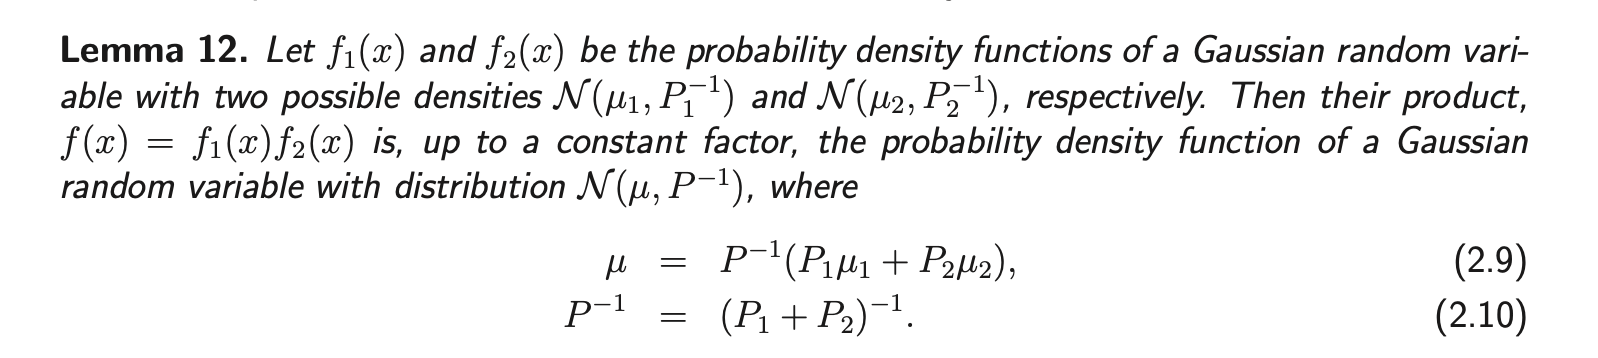
\includegraphics[width=\textwidth]{images/bickson_lemma_12}
\caption{Lemma 12 of \cite{bickson2008gaussian}}
\label{fig:lemma_twelve_bickson}
\end{figure}

\section{More on Bayesian multivariate linear regression}  \label{sec:more_bayesian_multivariate_linear_regression} 

Below we give an alternate proof for the posterior of the regression weights in multivariate linear regression,  compared to what was given in Proposition \ref{prop:bayes_linear_regression_with_known_ssq}.   This alternate proof may be of interest.   Whereas the proof of proposition \ref{prop:bayes_linear_regression_with_known_ssq} given in Section  \ref{sec:Bayesian_linear_regression_with_normal_prior} refers to exponential family properties,  the proof below does not,  and instead uses multivariate completing the square to do the heavy lifting. 

Note that proposition 
\ref{prop:bayes_linear_regression_with_known_ssq_and_zero_prior_mean} below, as stated,  is slightly more restrictive in that it assumes the prior mean is zero.   This additional restriction is not necessary; the proposition could be rewritten to match 
Proposition \ref{prop:bayes_linear_regression_with_known_ssq} exactly,  and the proof could be adjusted accordingly to match the additional generality.    The difference in statements is just an unnecessary presentational blemish.\redfootnote{TODO: fix up the unnecessary presentational blemish -- assuming that we don't end up sacrifing too much pedagogical clarity for the sake of generality}.
%The posterior distribution for \eqref{eqn:bayesian_multiple_linear_regression_with_known_observation_noise} is given by 

\begin{proposition} \label{prop:bayes_linear_regression_with_known_ssq_and_zero_prior_mean}
Consider the Bayesian linear multiple regression model
\begin{align*}
\+\beta &\sim \N (\+0, \+V) \\
y_i \cond \+\beta &\indsim \N (\+x_i^T \+\beta, \sigma^2),  \quad i=1,...,n
\end{align*}

where  $\+x_i$ designates the $i$-th row of the design matrix $\+X \in \R^{n \times p}$.

The posterior distribution for this model is given by 
\begin{align*}
p(\+\beta \cond \+y) & \sim \N(\+\mu,  \+\Sigma )
\intertext{where}
\+\mu &= \df{1}{\sigma^2} \+\Sigma \+X^T \+y \\
\+\Sigma &= \bigg( \df{1}{\sigma^2}  \+X^T \+X + \+V^{-1}  \bigg)^{-1} \\
\end{align*}
\end{proposition} 

\begin{proof}
The posterior on $\+\beta$ given $\+y = (y_1,...,y_N)^T$ is Gaussian,  since

\begin{align*}
\ln p(\+\beta \cond \+y) &= \ds\sum_{i=1}^n \ln p(y_i \cond \+\beta)  + \ln p(\+\beta) \\
&= -\df{1}{2 \sigma^2} \ds\sum_{i=1}^n (y_i - \+x_i^T \+\beta)^2  - \half \+\beta^T \+V^{-1} \+\beta + \text{constant} \\
&\stackrel{1}{=} -\df{1}{2 \sigma^2} \bigg(  \+y^T \+y - 2 \+y^T \+X^T \+\beta + \+\beta^T \+X^T \+X \+\beta \bigg)  - \half \+\beta^T \+V^{-1} \+\beta + \text{constant} \\
&\stackrel{2}{=} -\half (\+\beta - \+\mu)^T \+\Sigma^{-1} (\+\beta - \+\mu) +  \text{constant} \\
\intertext{where}  \\
\+\mu &= \df{1}{\sigma^2} \+\Sigma \+X^T \+y \\
\+\Sigma &= \bigg( \df{1}{\sigma^2}  \+X^T \+X + \+V^{-1}  \bigg)^{-1} \\
\end{align*}

Equality (1) is obtained by noting $ \sum_{i=1}^n (y_i - \+x_i^T \+\beta)^2  = (\+y - \+X \+\beta)^T (\+y - \+X \+\beta)$, FOIL-ing, and observing that the cross-products are scalars.   Equality (2) is obtained by completing the square,  where $\+\beta$ plays the role of $\+x$  in \eqref{eqn:multivariate_completing_the_square},  and where in that notation we have $\+M = \frac{1}{\sigma^2} \+X^T \+X + \+V^{-1}$ and $\+b^T = \frac{1}{\sigma^2} \+y^T \+X^T$
\end{proof}

\section{Matrix Facts}

\subsection{Multivariate completing the square}

A nice overview of multivariate completing the square is given by \cite{gundersenXXXXcompleting}.    

Let $\+x,  \+b$ be $d$-dimensional vectors, and let $\+M \in \R^{d \times d}$ be a symmetric invertible matrix. Then

\begin{align*}
\+x^T \+M \+x - 2 \+b^T \+x = (\+x - \+M^{-1} \+b)^T \+M (\+x - \+M^{-1} \+b) - \+b^T \+M^{-1} \+b
 \labelit \label{eqn:multivariate_completing_the_square}
\end{align*}

%  \+x^⊤ \+M \+x − 2\+b^⊤ \+x = (\+x−\+M^{−1} \+b)^T \+M (\+x−^\+M^{−1} \+b)− \+b^T \+M^{−1} \+b
% 

\subsection{The trace of a matrix product}

The trace of a matrix product behaves like a dot product.  

Let $\+A, \+B \in \R^{m \times n}$.  Then 

\begin{align*}
\tr (\+A^T \+B) = \ds\sum_{i=1}^n (\+A^T \+B)_i = \ds\sum_{i=1}^n \ds\sum_{j=1}^m a_{ij} b_{ij}
\labelit \label{eqn:trace_of_matrix_product}
\end{align*}

i.e.,  the trace of the matrix product is obtained by summing up the element-wise products. 


\section{The Inverse Wishart Distribution} \label{sec:inverse_wishart_distribution}
 
The Inverse Wishart is a distribution on symmetric,  positive definite matrices.     The Inverse Wishart distribution,  denoted $\InverseWishart(\nu, \+\Psi)$,  has density

\begin{align}
p(\+\Sigma) \propto | \+\Sigma|^{-(\nu+d +1) /2}  \exp \bb{ -\df{1}{2} \tr ( \+\Sigma^{-1} \+\Psi) } 
\label{eqn:inverse_wishart_density}
\end{align}
where $\+\Sigma \succ 0$ and $\nu > d-1$ to have a proper prior.     The expected value of an Inverse Wishart random variable parametrized as in \eqref{eqn:inverse_wishart_density} is given by $\E[\+\Sigma] = \frac{\+\Psi}{\nu -d -1}$.   

\begin{remark}{\remarktitle{Interpreting the parameters of the Inverse Wishart}}
\label{rk:inverse_wishart_parameter_interpretation}
Note that the parameters of the Inverse Wishart can be interpreted (as per conjugacy;  see \eqref{eqn:Sigma_cc_normal_model_cond_conj_prior}) in the following way: the covariance was estimated from $\nu$ observations with a residual sum of squares (a.k.a.  sum of pairwise deviation products) $\+\Psi$. 
\qed
\end{remark}

Remark \ref{rk:inverse_wishart_parameter_interpretation} also provides inuition on the expected value.      For a visualization of how samples are affected by the parameters,  see \cite{hughesXXXXinverse}. 

\begin{remark}{\remarktitle{Peter Hoff's notation for the Inverse Wishart: A warning}}
\label{rk:peter_hoffs_notation_for_inverse_wishart}
Note that some authors (e.g.  \cite{hoff2009first},  pp.257) use the notation $\InverseWishart(\nu,  \+M)$ to refer to the density under reparametrization
\begin{align}
p(\+\Sigma) \propto | \+\Sigma|^{-(\nu+d +1) /2}  \exp \bb{ -\df{1}{2} \tr ( \+\Sigma^{-1} \+M^{-1}) } 
\label{eqn:inverse_wishart_density_hoff}
\end{align}
and therefore appropriately altered normalization constant.  The expected value of an Inverse Wishart random variable parametrized as in   \eqref{eqn:inverse_wishart_density_hoff},  is given by $\E[\+\Sigma] = \frac{\+M^{-1}}{\nu -d -1}$.     

However,  Hoff later introduces the reparametrization $\+S := \+M^{-1}$,  and so writes $\InverseWishart(\nu, \+S^{-1})$ to mean 
\begin{align}
p(\+\Sigma) \propto | \+\Sigma|^{-(\nu+d +1) /2}  \exp \bb{ -\df{1}{2} \tr ( \+\Sigma^{-1} \+S) } 
\label{eqn:inverse_wishart_density_hoffs_alternate}
\end{align}
which is \eqref{eqn:inverse_wishart_density}, and which we would write as $\InverseWishart(\nu, \+S)$.
\qed
\end{remark}

\begin{remark}{\remarktitle{Comparing parametrizations}}
Regarding Remark \ref{rk:peter_hoffs_notation_for_inverse_wishart},  prefer our notation because 
\begin{itemize}
\item It is the natural parameterization (see Example \ref{ex:inverse_wishart_as_ef}).
\item It lets $\+\Psi$ be interpreted directly as a prior residual sum of squares (see Remark \ref{rk:inverse_wishart_parameter_interpretation}). 
\item It matches the parametrization used throughout Wikipedia,  e.g. in its conjugacy tables.
\end{itemize}
\qed
\end{remark}

The  Inverse Wishart is a popular choice for modeling covariance matrices (e.g.  see \cite{hoff2009first}),  due to at least the fact that is a  conditionally conjugate prior on the covariance of a normal distribution.   (See Section \ref{sec:normal_data_with_non_conjugate_prior}.)   It seems to me that a weakly informative prior could be constructed by setting  $\nu = d+2$ (the smallest integer for which $\nu$ is in the parameter space) and $\+\Psi = (\nu -d - 1) \+I = \+I$.   This would presumably be reasonable at least if one expected unit variances and wanted to make a prior assumption of independence across dimensions.

Some problems with the Inverse Wishart as a model for covariance matrices is summarized in  \cite{alvarez2014bayesian}.    We highlight that:
\begin{enumerate}
\item  When $\nu  > 1$,   the implied scaled inv-$\chi^2$ distribution on the individual variances has extremely low density in the region near zero.   
\item The prior imposes a dependency between the correlations and the variances. In particular,  larger variances are associated with absolute values of the correlations near 1 while small variances
are associated with correlations near zero.    
\end{enumerate}
For additional discussion on the problems with Inverse Wishart,  especially when used in hierarchical models,  and for a remedy using a half-t distribution that also has a conditionally conjugate construction,  see \cite{wojnowiczXXXXcategorical}.

The Wishart distribution has the same support as the Inverse Wishart;  however,  the Wishart does not give a conditionally conjugate prior on the covariance of a normal distribution.    The Inverse Wishart density can be derived from the Wishart via the multivariate change of variables  \cite{wolpert2011change}. \footnote{It is claimed in Wikipedia that if $\+X \sim \Wishart(\nu,  \+\Psi)$  then $\+X^{-1} \sim \InverseWishart(\nu,  \+\Psi^{-1})$.   I almost was able to show this using the multivariate change of variables  \cite{wolpert2011change} along with (15.15) of \cite{dwyer1967some},  but I  was off by a negative when attempting to combine the two terms with $|\+X^{-1}|$ raised to an exponent.}\redfootnote{TO DO: Provide derivation.}

A sample $\+\Sigma$ from the $\InverseWishart(\nu, \+\Psi)$ distribution (using the natural parametrization of \eqref{eqn:inverse_wishart_density}) can be obtained by the following scheme\redfootnote{TODO: Provide derivation of this scheme.  See perhaps \url{https://www.math.wustl.edu/~sawyer/hmhandouts/Wishart.pdf}.} \cite{hoff2009first}:

\begin{enumerate}
\item Sample $\+z_1, ..., \+z_{\nu} \iid \N (\+0,  \+\Psi^{-1})$
\item Calculate $\+Z^T \+Z = \sum_{i=1}^\nu \+z_i \+z_i^T$.
\item Set $\+\Sigma = ( \+Z^T \+Z )^{-1}$.
\end{enumerate}
The intuition is that the Inverse Wishart models covariance matrices as an inverse sum of squares (again, see Remark \ref{rk:inverse_wishart_parameter_interpretation}).  

The inverse Wishart can be seen as a generalization of the inverse gamma distribution to multiple dimensions.\redfootnote{TODO: fill in.   Make explicit how it is a generalization.}


\bibliography{references_exponential_family}{}
\bibliographystyle{unsrt}


\end{document}